\documentclass[a4paper]{ctexart}
\usepackage{xeCJK}
\usepackage{setspace}
\usepackage{graphicx,wrapfig}
\usepackage{fontspec,xunicode,xltxtra}
\usepackage{fancyhdr,titlesec,titletoc}
\usepackage[titletoc]{appendix}
\usepackage[top=29mm,bottom=29mm,left=31.8mm,right=31.8mm]{geometry}
\usepackage{enumerate,enumitem}
\usepackage{caption}
\usepackage{amsmath,amssymb,bm,array}
\usepackage{cite}
\usepackage{diagbox}
\usepackage{algorithm,algorithmicx,algpseudocode}
\usepackage{multirow}
\usepackage{listings}
\usepackage{color}
\setmainfont{Times New Roman}
\setCJKmainfont[BoldFont={Songti SC Bold}]{SimSun}
\setCJKfamilyfont{heiti}{SimHei}
\renewcommand{\heiti}{\CJKfamily{heiti}\fontspec{Times New Roman}}

\newcommand{\mycaptionfont}{\heiti\zihao{5}}
\captionsetup[figure]{name={\mycaptionfont 图},labelsep=period}
\captionsetup[table]{name={\mycaptionfont 表},labelsep=period}
\floatname{algorithm}{\mycaptionfont 算法}
\captionsetup[algorithm]{labelsep=period}
\renewcommand{\captionfont}{\mycaptionfont}
\renewcommand{\captionlabelfont}{\mycaptionfont}

\ctexset {
	section = {
		number = \arabic{section},
		format = \zihao{4}\bfseries,
	},
	subsection = {
		number = \arabic{section}.\arabic{subsection},
		format = \zihao{-4}\bfseries,
	},
	subsubsection = {
		number = \arabic{section}.\arabic{subsection}.\arabic{subsubsection},
		format = \zihao{-4}\bfseries,
	}
}
\setlist[enumerate]{itemindent=2em,listparindent=2em,leftmargin=1em,label=\arabic*、}

\setlength\parskip{.5\baselineskip}
\fancypagestyle{plain}{\pagestyle{fancy}}%改变章节首页页眉
\pagestyle{fancy}
\lhead{\kaishu~嵌入式系统课程设计~}
\rhead{\kaishu~1030616134~尹达恒~}
\cfoot{\thepage}

\definecolor{codegreen}{rgb}{0,0.6,0}
\definecolor{codegray}{rgb}{0.5,0.5,0.5}
\definecolor{codepurple}{rgb}{0.58,0,0.82}
\definecolor{backcolour}{rgb}{0.95,0.95,0.92}

\titlecontents{section}[0em]{\vspace{0.01\baselineskip}\songti\zihao{-4}}{\thecontentslabel\ }{}
{\hspace{.5em}\titlerule*[4pt]{$\cdot$}\contentspage}
\titlecontents{subsection}[2em]{\vspace{0.01\baselineskip}\songti\zihao{-4}}{\thecontentslabel\ }{}
{\hspace{.5em}\titlerule*[4pt]{$\cdot$}\contentspage}
\setcounter{tocdepth}{2}

\begin{document}

\lstset{
	language={C},
	numbers=left,numberstyle=\tiny,
	basicstyle=\small\ttfamily,
	stringstyle=\color{codepurple},
	keywordstyle=\color{blue}\bfseries,
	commentstyle=\color{codegreen},
	rulesepcolor=\color{codegray},
	tabsize=2
}

\begin{spacing}{1}
\tableofcontents
\end{spacing}
\newpage

\begin{center}
	{\zihao{-3}\textbf{基于$\bm\mu$C/OS-II的流水灯按键控制系统设计}}

	{\zihao{-4}尹达恒}\\[-1mm]

	{\zihao{5}(江南大学物联网工程学院,江苏\quad 无锡)}
\end{center}
\begin{spacing}{1.3}
	\songti\zihao{-4}
	\section{设计要求}
	\begin{itemize}
		\item 利用P0口的一个管脚作为一个按键信号输入,其作用是启动流水灯的开始和停止(第一次按启动,第二次停止,第三次启动,以此类推);
		\item 利用P0口的一个管脚作为一个按键信号输入,其作用是设置灯亮的时间,分三档1秒,2秒,3秒(第一次按1,第二次2秒,第三次3秒,第四次1秒,以此类推);
		\item 基于$\mu$C/OS-II操作系统,完成以上程序设计。
	\end{itemize}

	\section{设计原理}
	\subsection{LED流水灯运行原理}
	LED流水灯实际上就是八个LED。如果要点亮一个阴极接地的LED,需要在其阳极接入高电平;相反, 如果要让这个LED熄灭,就要阳极接入低电平。因此,要实现流水灯功能,只要在八个LED的阳极依次接入高电平,八个LED灯便会一亮一暗的做流水灯了。另外,由于人眼的视觉暂留效应以及单片机执行每条指令的时间很短,在控制二极管亮灭的时候应该延时一段时间。

	\subsection{按键控制原理}
	按键的基本原理是读取单片机IO口的输入状态。对于一个接地按键来说,当IO口输入低于某一阈值时表明按键按下,此时在STM32的程序中可以读取到对应的IO口值为0。根据不同时刻IO口的01值即可获得按键状态,并以此控制单片机的行为。
	
	\subsection{$\bm\mu$C/OS-II操作系统运行原理}
	$\mu$C/OS-II由Micrium公司提供,是一个可移植、可固化的、可裁剪的、占先式多任务实时内核,它适用于多种微处理器,微控制器和数字处理芯片$\mu$C/OS-II可以大致分成核心、任务处理、时间处理、任务同步与通信和CPU接口5个部分:
	\begin{itemize}
		\item 核心部分:操作系统的处理核心,包括操作系统初始化、操作系统运行、中断进出的前导、时钟节拍、任务调度、事件处理等功能代码;
		\item 任务处理部分:任务处理部分中的内容都是与任务的操作密切相关的。包括任务的建立、删除、挂起、恢复等;
		\item 时钟部分:$\mu$C/OS-II中的最小时钟单位是timetick(时钟节拍)。任务延时等操作是在时钟部分完成;
		\item 任务同步和通信部分:为事件处理部分,包括信号量、邮箱、邮箱队列、事件标志等部分;主要用于任务间的互相联系和对临界资源的访问;
		\item CPU接口部分:主要包括中断级任务切换的底层实现、任务级任务切换的底层实现、时钟节拍的产生和处理、中断的相关处理部分等内容。由于$\mu$C/OS-II是一个通用性的操作系统,所以对于关键问题上的实现,还是需要根据具体CPU的具体内容和要求作相应的移植。这部分内容由于牵涉到SP等系统指针,所以用汇编语言编写。主要的移植工作都在此部分进行。
	\end{itemize}

	\section{设计方案}
	\subsection{硬件设计}\label{硬件设计}
	根据设计要求,流水灯按键控制系统设计方案的硬件主要包含以下部分:
	\begin{itemize}
		\item STM32单片机最小系统;
		\item 两个按键;
		\item 八个LED。
	\end{itemize}
	
	并使用STM32 GPIOB的高八位管脚控制LED,低八位管脚获取按键状态。

	\subsection{软件设计}\label{软件设计}
	根据设计要求,流水灯按键控制系统的软件包含两个标志位和两个进程:
	\begin{itemize}
		\item 启停标志位:无符号整数,该标志位为奇数时流水灯保持运行,为偶数时流水灯暂停运行;
		\item 速度标志位:无符号整数,流水灯运行速度为(速度标志位mod 3)秒/位,当速度标志位发生变化时改变流水灯的运行速度;
		\item 按键进程:每隔一定时间扫描按键状态,并按照按键状态改变标志位值;
		\item 流水进程:每隔一定时间检查标志位值,并按照标志位值改变LED的亮灭状态。
	\end{itemize}
	

	\section{系统实现}
	\subsection{硬件实现}
	开发板使用PERCHIN HC6800-EM3,其核心板芯片为STM32F103C8T6,最小系统电路图如附录\ref{apdx:最小系统原理图}、接地按键电路如图\ref{fig:按键}、LED电路如图\ref{fig:LED}。使用杜邦线将最小系统的PB0$\sim$PB7和PB8$\sim$PB15分别与按键电路的JP5和J12相连,从而使得GPIOB的高八位管脚连接LED,低八位管脚连接按键。
	\begin{figure}[htbp]
		\centering
		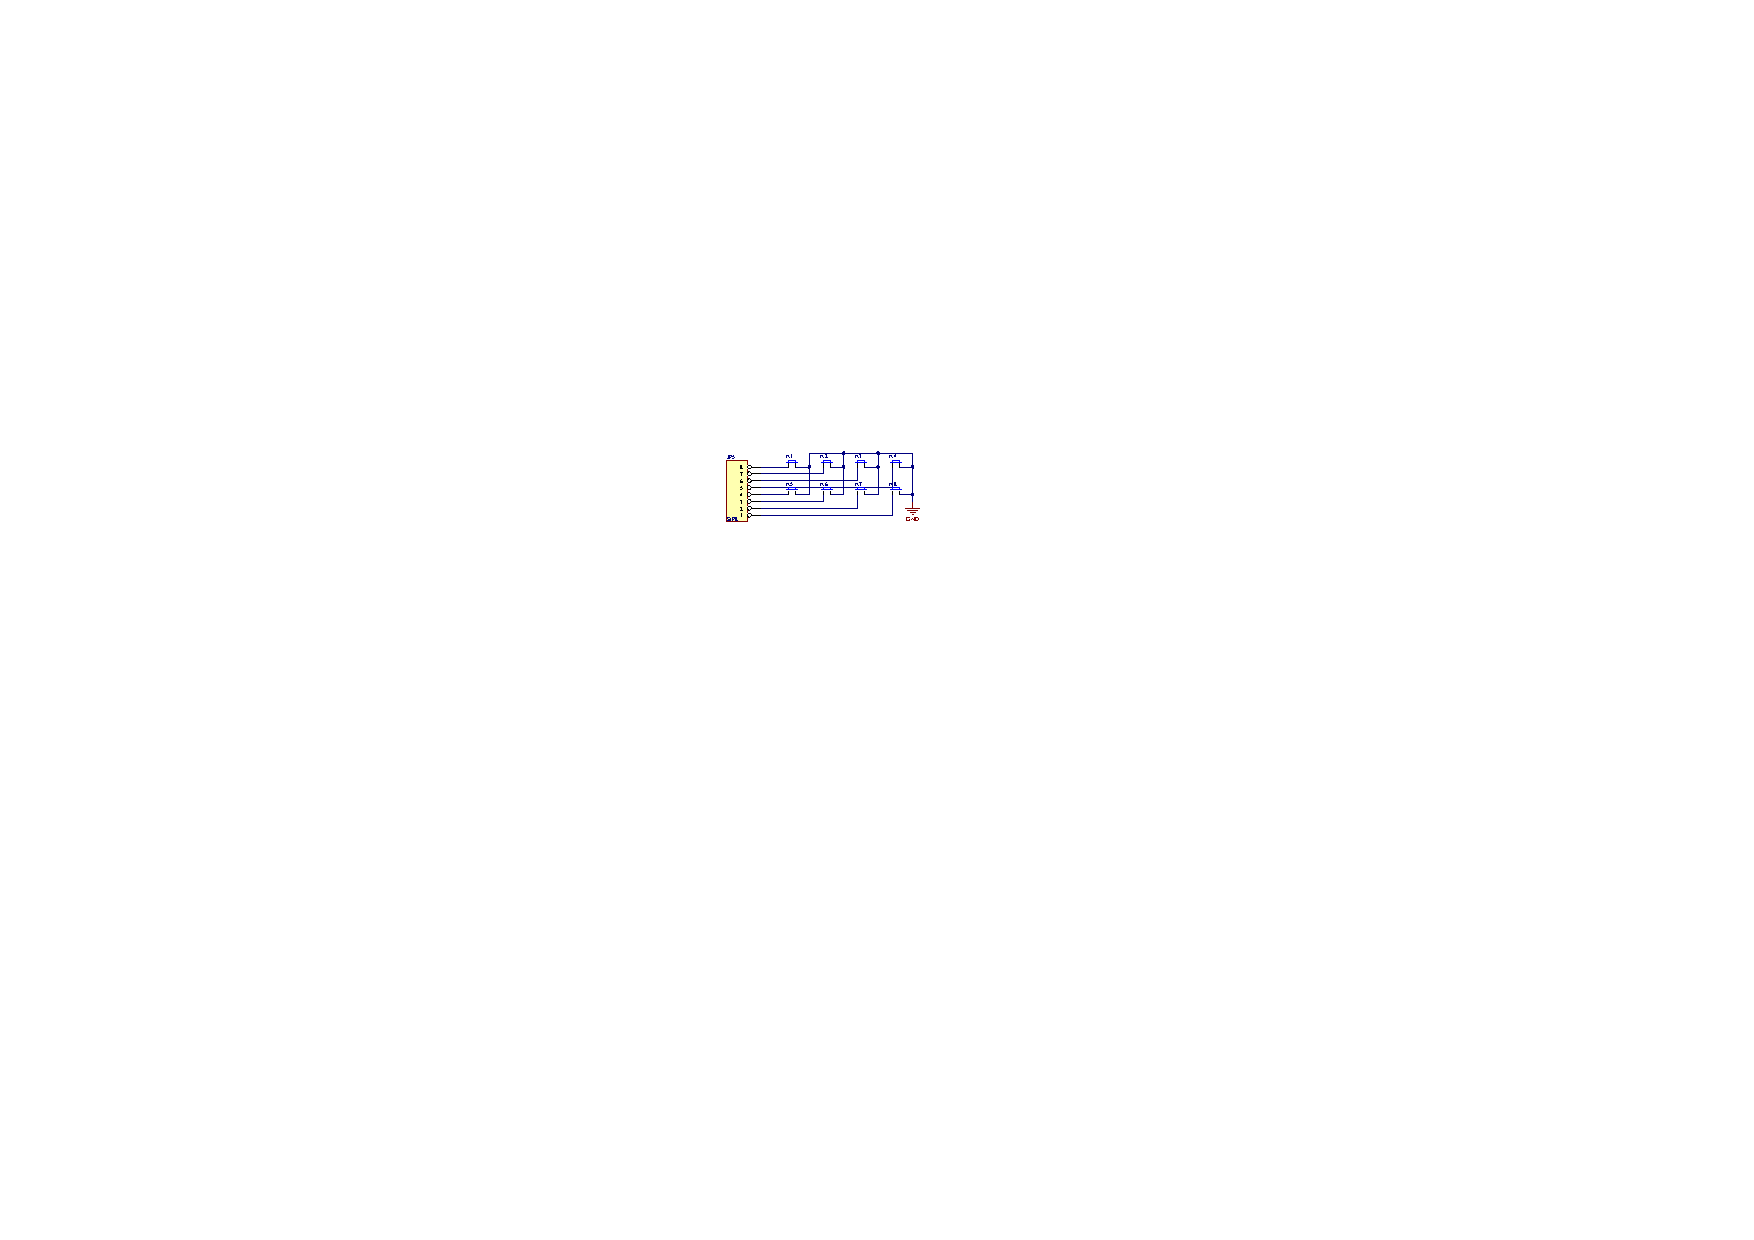
\includegraphics[width=\textwidth]{figure/KEY.pdf}
		\caption{按键电路原理图(使用其中的K7、K8按键)}\label{fig:按键}
	\end{figure}
	\begin{figure}[htbp]
		\centering
		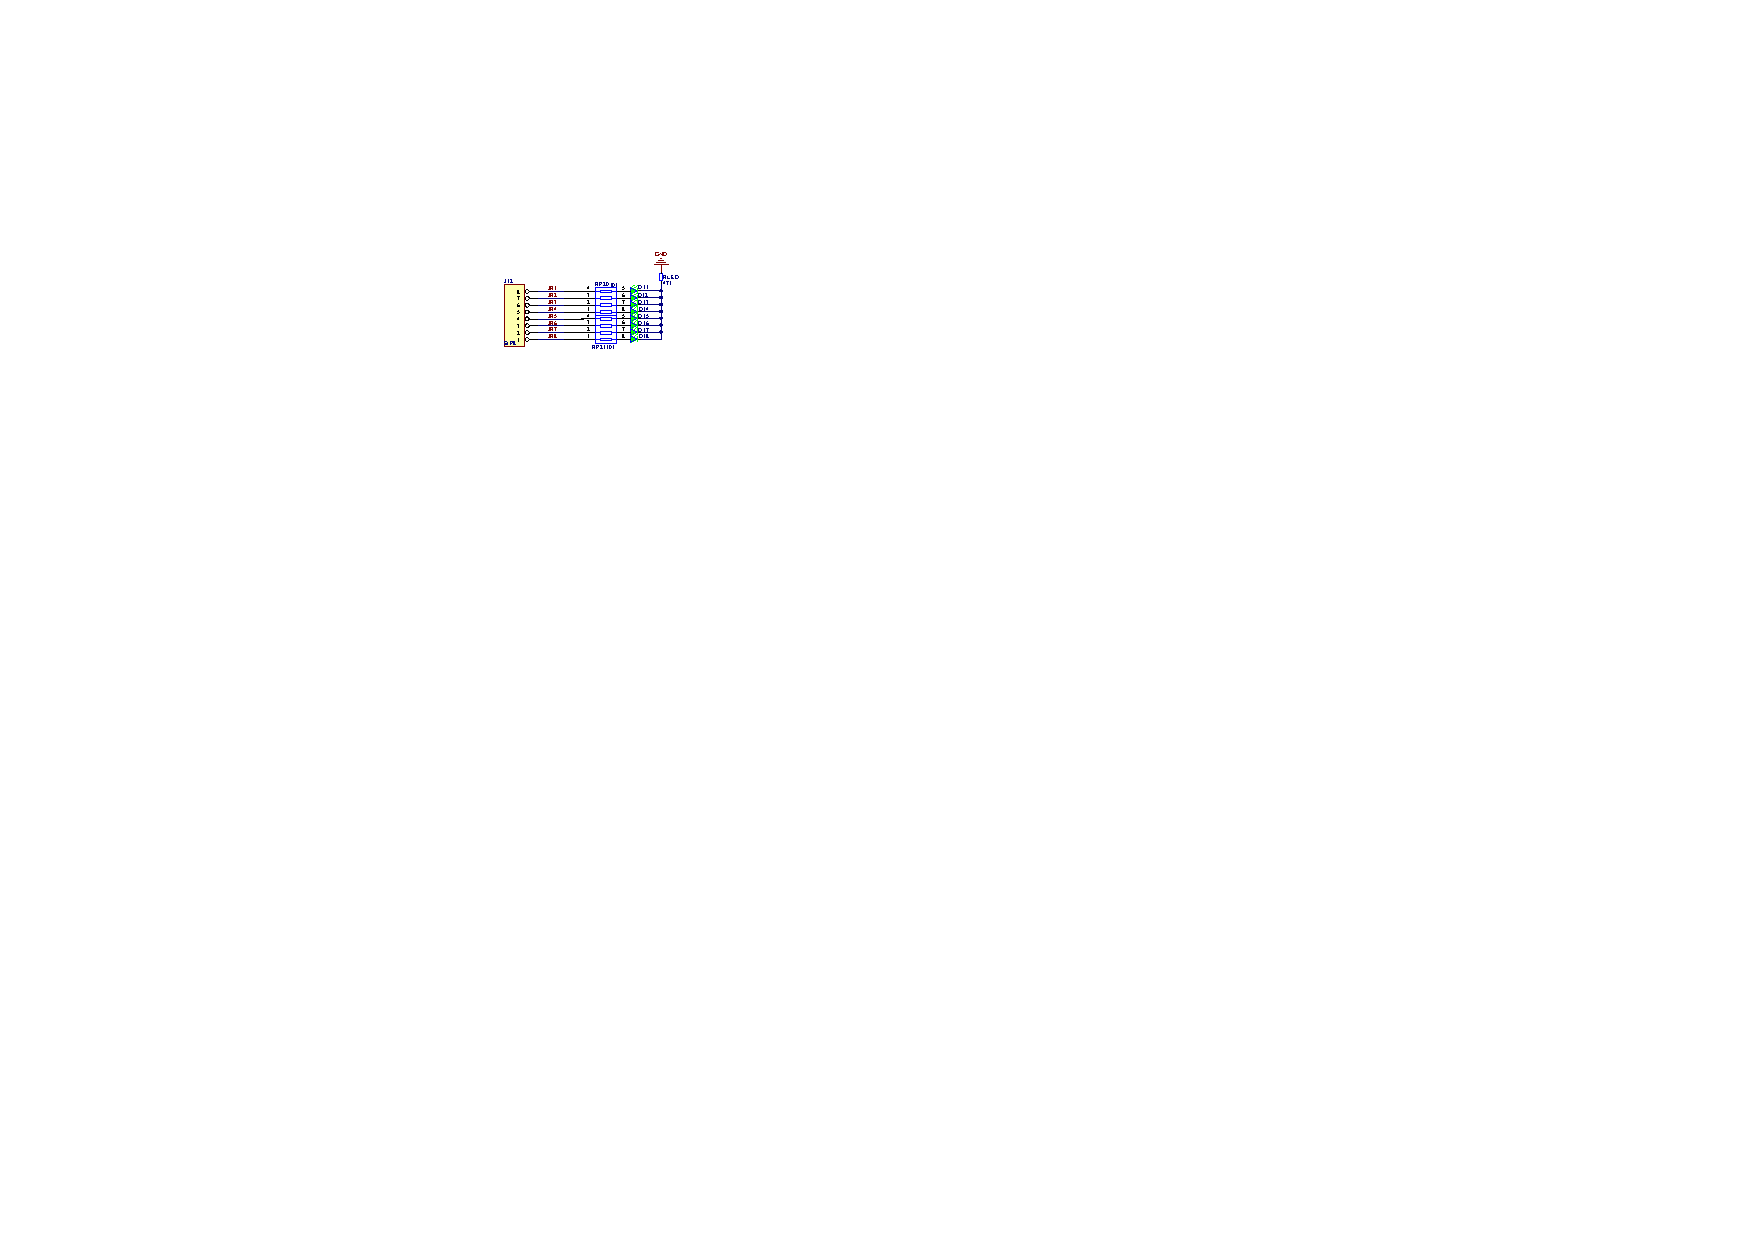
\includegraphics[width=\textwidth]{figure/LED.pdf}
		\caption{LED电路原理图}\label{fig:LED}
	\end{figure}

	\subsection{软件实现}
	\subsubsection{$\bm\mu$C/OS-II移植}\label{uCOS移植}
	$\mu$C/OS-II的详细移植步骤如下:
	\begin{enumerate}[label=\arabic*、]
		\item 构造一个裸机Demo,实现基本的流水灯;
		\item 至Micrium官网下载并解压STM32F107官方移植的$\mu$C/OS,其中Keil MDK4的版本是$\mu$C/OS 2.92.07;
		\item 将下列文件夹中的文件复制到裸机Demo下:
		\begin{itemize}
			\item Micrium/Software/uCOS-II/Ports
			\item Micrium/Software/uCOS-II/Source
			\item Micrium/Software/EvalBoards/Micrium/uC-Eval-STM32F107/uCOS-II中的\newline os\_cfg.h、app\_cfg.h、app\_hooks.c、includes.h。
		\end{itemize}
		\item 在Keil工程中添加上一步中复制的文件;
		\item 修改includes.h:删去bsp(Board Support Pack,开发板支持)和lib相关的include引用;
		\item 修改stm32f10x\_it.c:
		\begin{itemize}
			\item 在SysTick中断处理函数SysTick\_Handler()中调用操作系统的SysTick函数OS\_CPU\_SysTickHandler();
			\item 删去原有的PendSV异常处理函数PendSV\_Handler(),防止下一步中修改uCOS的os\_cpu\_a.asm后出现重定义错误;
		\end{itemize}
		\item 修改os\_cpu\_a.asm:
		\begin{itemize}
			\item 将操作系统原有的PendSV处理函数OS\_CPU\_PendSVHandler重命名为PendSVHandler;
			\item 将文件开头的EXPORT OS\_CPU\_PendSVHandler改为EXPORT PendSVHandler。
		\end{itemize}
	\end{enumerate}
	\subsubsection{按键进程函数}\label{按键进程}
	\begin{itemize}
		\item 编写函数KEY\_gets(),使用一个全局变量保存按键状态,在KEY\_gets()中调用GPIO\_ReadInputData读取当前按键状态(8位二进制数),若当前按键状态与保存的按键状态不同且为按下状态,即表明按键经历了一个按下的过程,此时KEY\_gets()返回值对应位置1,否则返回0;
		\item 编写按键进程函数LED\_change(),该函数的while循环每隔10毫秒运行一次,在循环中调用KEY\_gets()函数获取按键状态并判定按下的按键,如果按下了按键K8,则改变启停标志位值;如果按下了按键K7,则改变速度标志位值。
	\end{itemize}

	按键进程的运行流程可以用如图\ref{fig:KEY流程图}所示的流程图表示。核心代码如附录\ref{按键进程代码}。

	\begin{figure}[htbp]
		\centering
		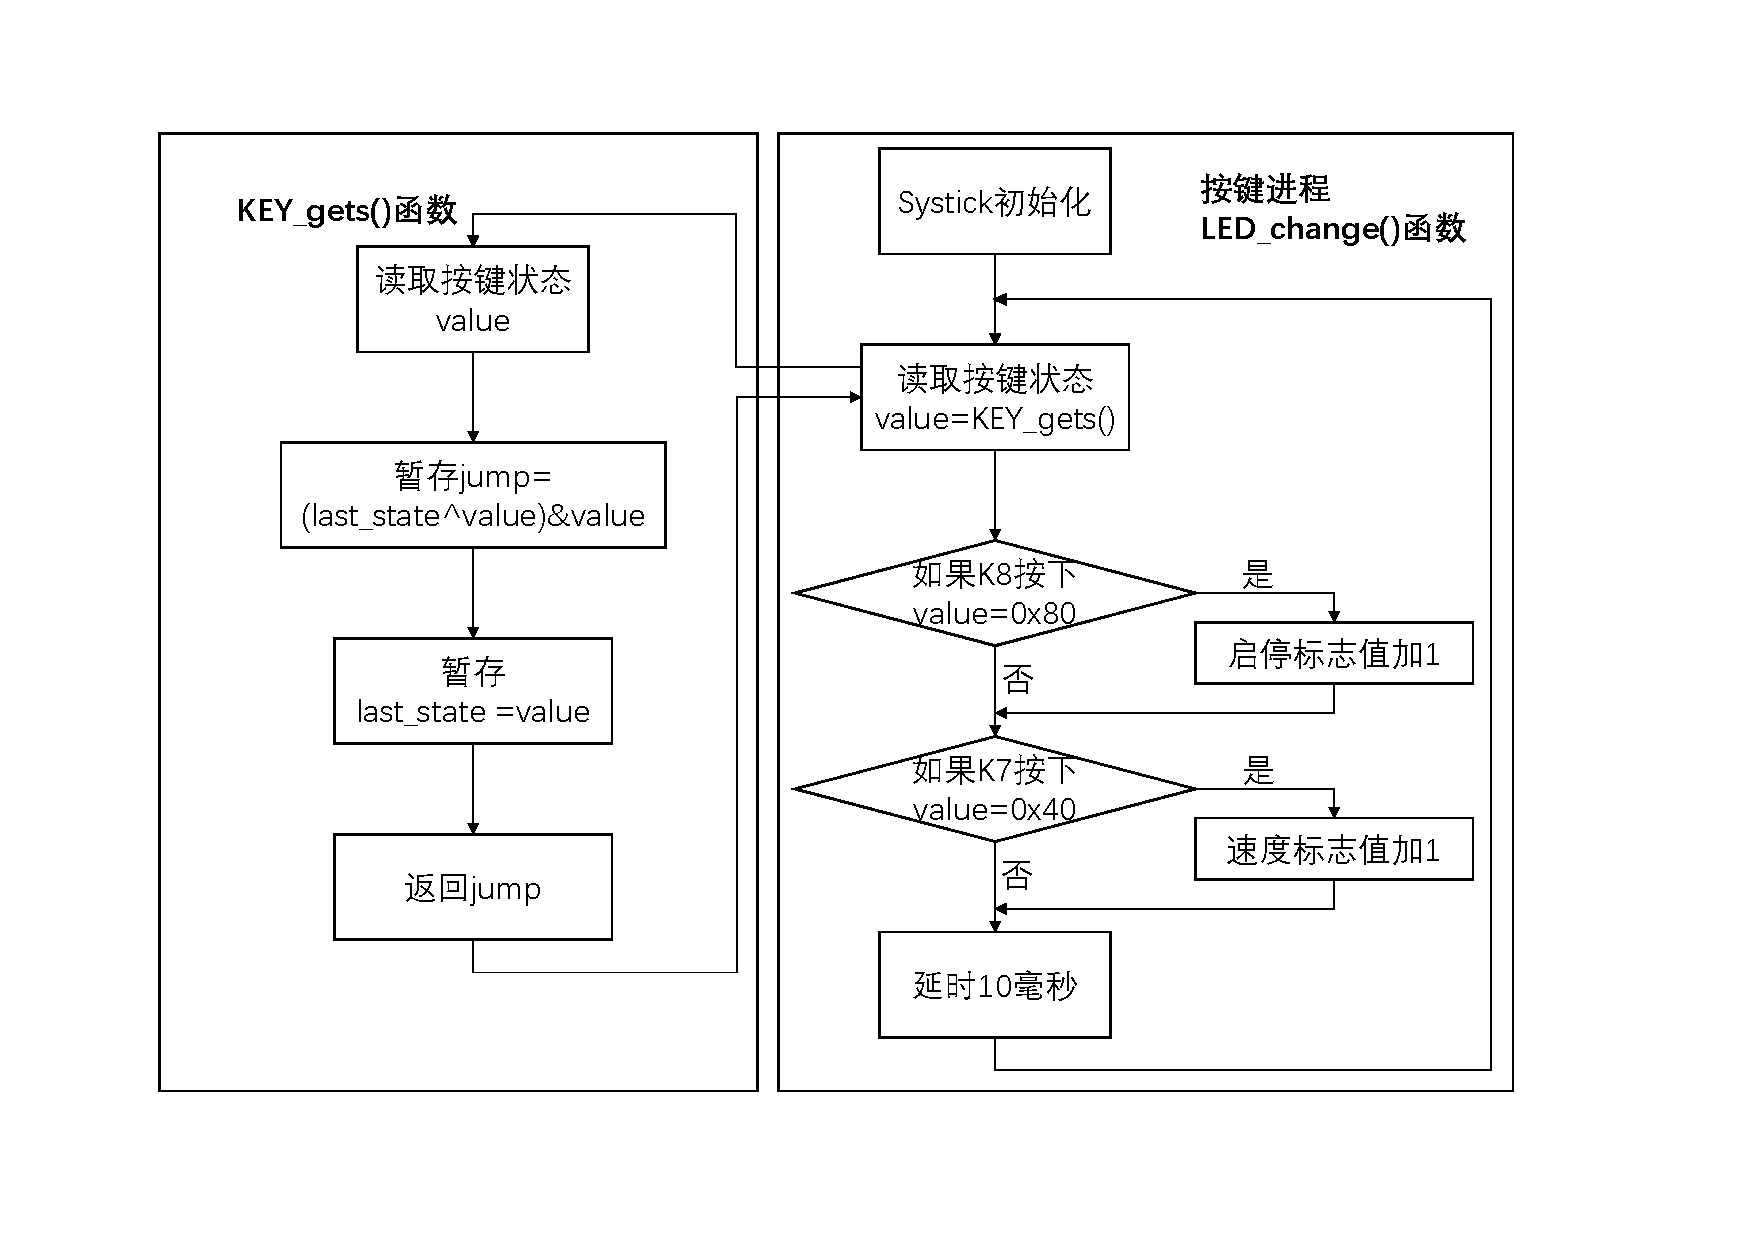
\includegraphics[width=\textwidth]{figure/KEYflow.pdf}
		\caption{按键进程流程图}\label{fig:KEY流程图}
	\end{figure}

	\subsubsection{流水进程函数}\label{流水进程}
	流水进程由一个while循环构成,每次循环中都会进行如下操作:
	\begin{itemize}
		\item 读取启停标志位的值,若该值为奇数,则调用LED\_Sets函数亮起流水灯中的下一个灯,否则不进行任何操作;
		\item 读取速度标志位的值,以该值的模3余数加一为秒数,调用OSTimeDlyHMSM函数设置下一次循环的运行时间。
	\end{itemize}

	流水进程的运行流程可以用如图\ref{fig:LED流程图}所示的流程图表示。核心代码如附录\ref{流水进程代码}。

	\begin{figure}[htbp]
		\centering
		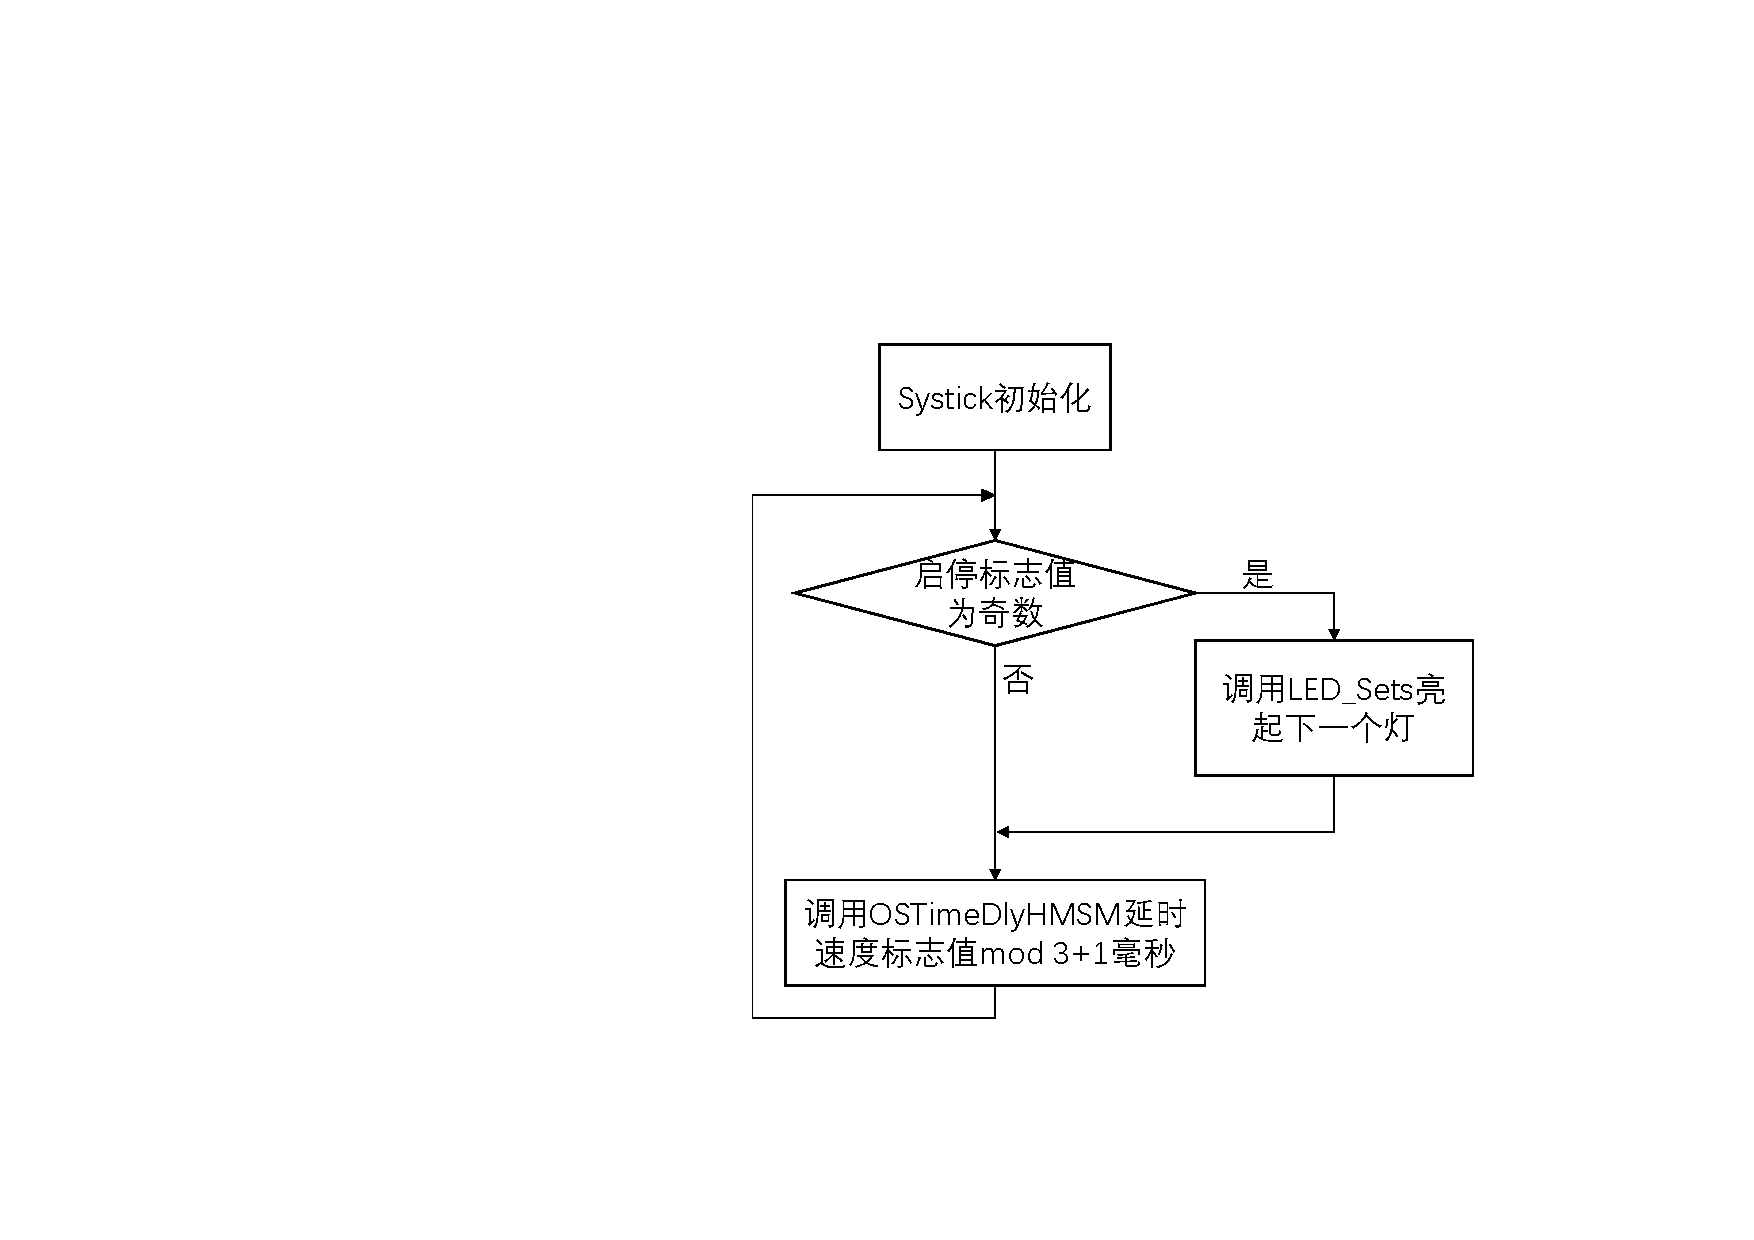
\includegraphics[width=0.5\textwidth]{figure/LEDflow.pdf}
		\caption{流水灯进程流程图}\label{fig:LED流程图}
	\end{figure}

	\subsubsection{主函数}
	在主函数中需要进行系统时钟、管脚和操作系统的初始化操作以及操作系统的任务创建和启动,相关核心代码如附录\ref{主函数代码}所示,各部分实现流程如下:
	\begin{itemize}
		\item 系统时钟初始化:使用系统固件库函数RCC\_GetClocksFreq获取到系统时钟源HCLK的频率;调用SysTick设置函数SysTick\_Config设置systick重装定时器的值=HCLK频率/操作系统每秒钟的Tick数OS\_TICKS\_PER\_SEC,使操作系统获取到准确的系统时钟;
		\item 管脚的初始化:根据\ref{硬件设计}节中的设计方案,需要将GPIOB管脚高八位设置为推挽输出,低八位设置为上拉输入。使用GPIO\_InitStructure结构和GPIO\_Init函数进行设置;
		\item 操作系统系统的初始化:$\mu$C/OS-II操作系统的初始化通过调用函数OSInit()完成;
		\item 操作系统任务的创建:根据\ref{软件设计}节中的设计方案,需要调用OSTaskCreate函数将\ref{按键进程}节中编写的按键进程函数和\ref{流水进程}流水进程函数分别创建为两个进程,且使流水进程的优先级为最高,从而获得较为准确的定时时间;
		\item 操作系统的启动:$\mu$C/OS-II操作系统的启动通过调用函数OSStart()函数完成。
	\end{itemize}
	
	\section{设计结果与总结}
	\subsection{设计结果}
	编译工程并下载至开发板芯片中查看实现效果,其结果完全符合设计要求,当按下按键K8时,流水灯以每2秒一次的速度启动,此时按键K8控制流水灯的暂停和继续;流水灯的速度受到按键K7的控制,每次按下K7按键时,流水灯的速度都会在1秒一次$\rightarrow$2秒一次$\rightarrow$3秒一次三个状态之间循环。

	\subsection{遇到的问题}
	\subsubsection*{汇编函数OS\_CPU\_PendSVHandler的调用问题}
	\begin{itemize}
		\item 问题描述:在\ref{uCOS移植}节介绍的移植过程中,os\_cpu\_a.asm中的OS\_CPU\_PendSVHandler函数需要在作为可挂起系统中断函数在PendSV中断时进行调用,但若将其放入stm32f10x\_it.c文件的PendSV\_Handler中系统无法正常工作。
		\item 问题原因:OS\_CPU\_PendSVHandler的作用是在时间片轮转和系统出错时保存现场,因此使用汇编语言编写,而若将其放在PendSV\_Handler中作为一个函数进行调用,在编译过后,其保存的现场为PendSV\_Handler中断处理函数的现场,而不是正常程序执行时的现场,因此系统无法正常工作。
		\item 问题解决:直接在os\_cpu\_a.asm中将OS\_CPU\_PendSVHandler函数名称修改为PendSV\_Handler,使得PendSV中断发生时直接调用os\_cpu\_a.asm的处理函数。
	\end{itemize}

	\subsection{心得体会}
	\begin{itemize}
		\item 巩固了单片机和嵌入式系统的课程知识,更加深入地理解了单片机和嵌入式系统的工作原理;
		\item 实际看到了一个简单操作系统的实现代码,更加深入地理解了操作系统的工作流程和实现方法,尤其是任务调度和保存现场的过程;
		\item 进一步精进了代码水平,对嵌入式系统的开发更加熟练。
	\end{itemize}

\end{spacing}
\newpage
\section*{附录}\addcontentsline{toc}{section}{附录}\appendix
\section{STM32F103C8T6最小系统原理图(PRECHIN STM32核心板)}\label{apdx:最小系统原理图}
\begin{figure}[htbp]
	\centering
	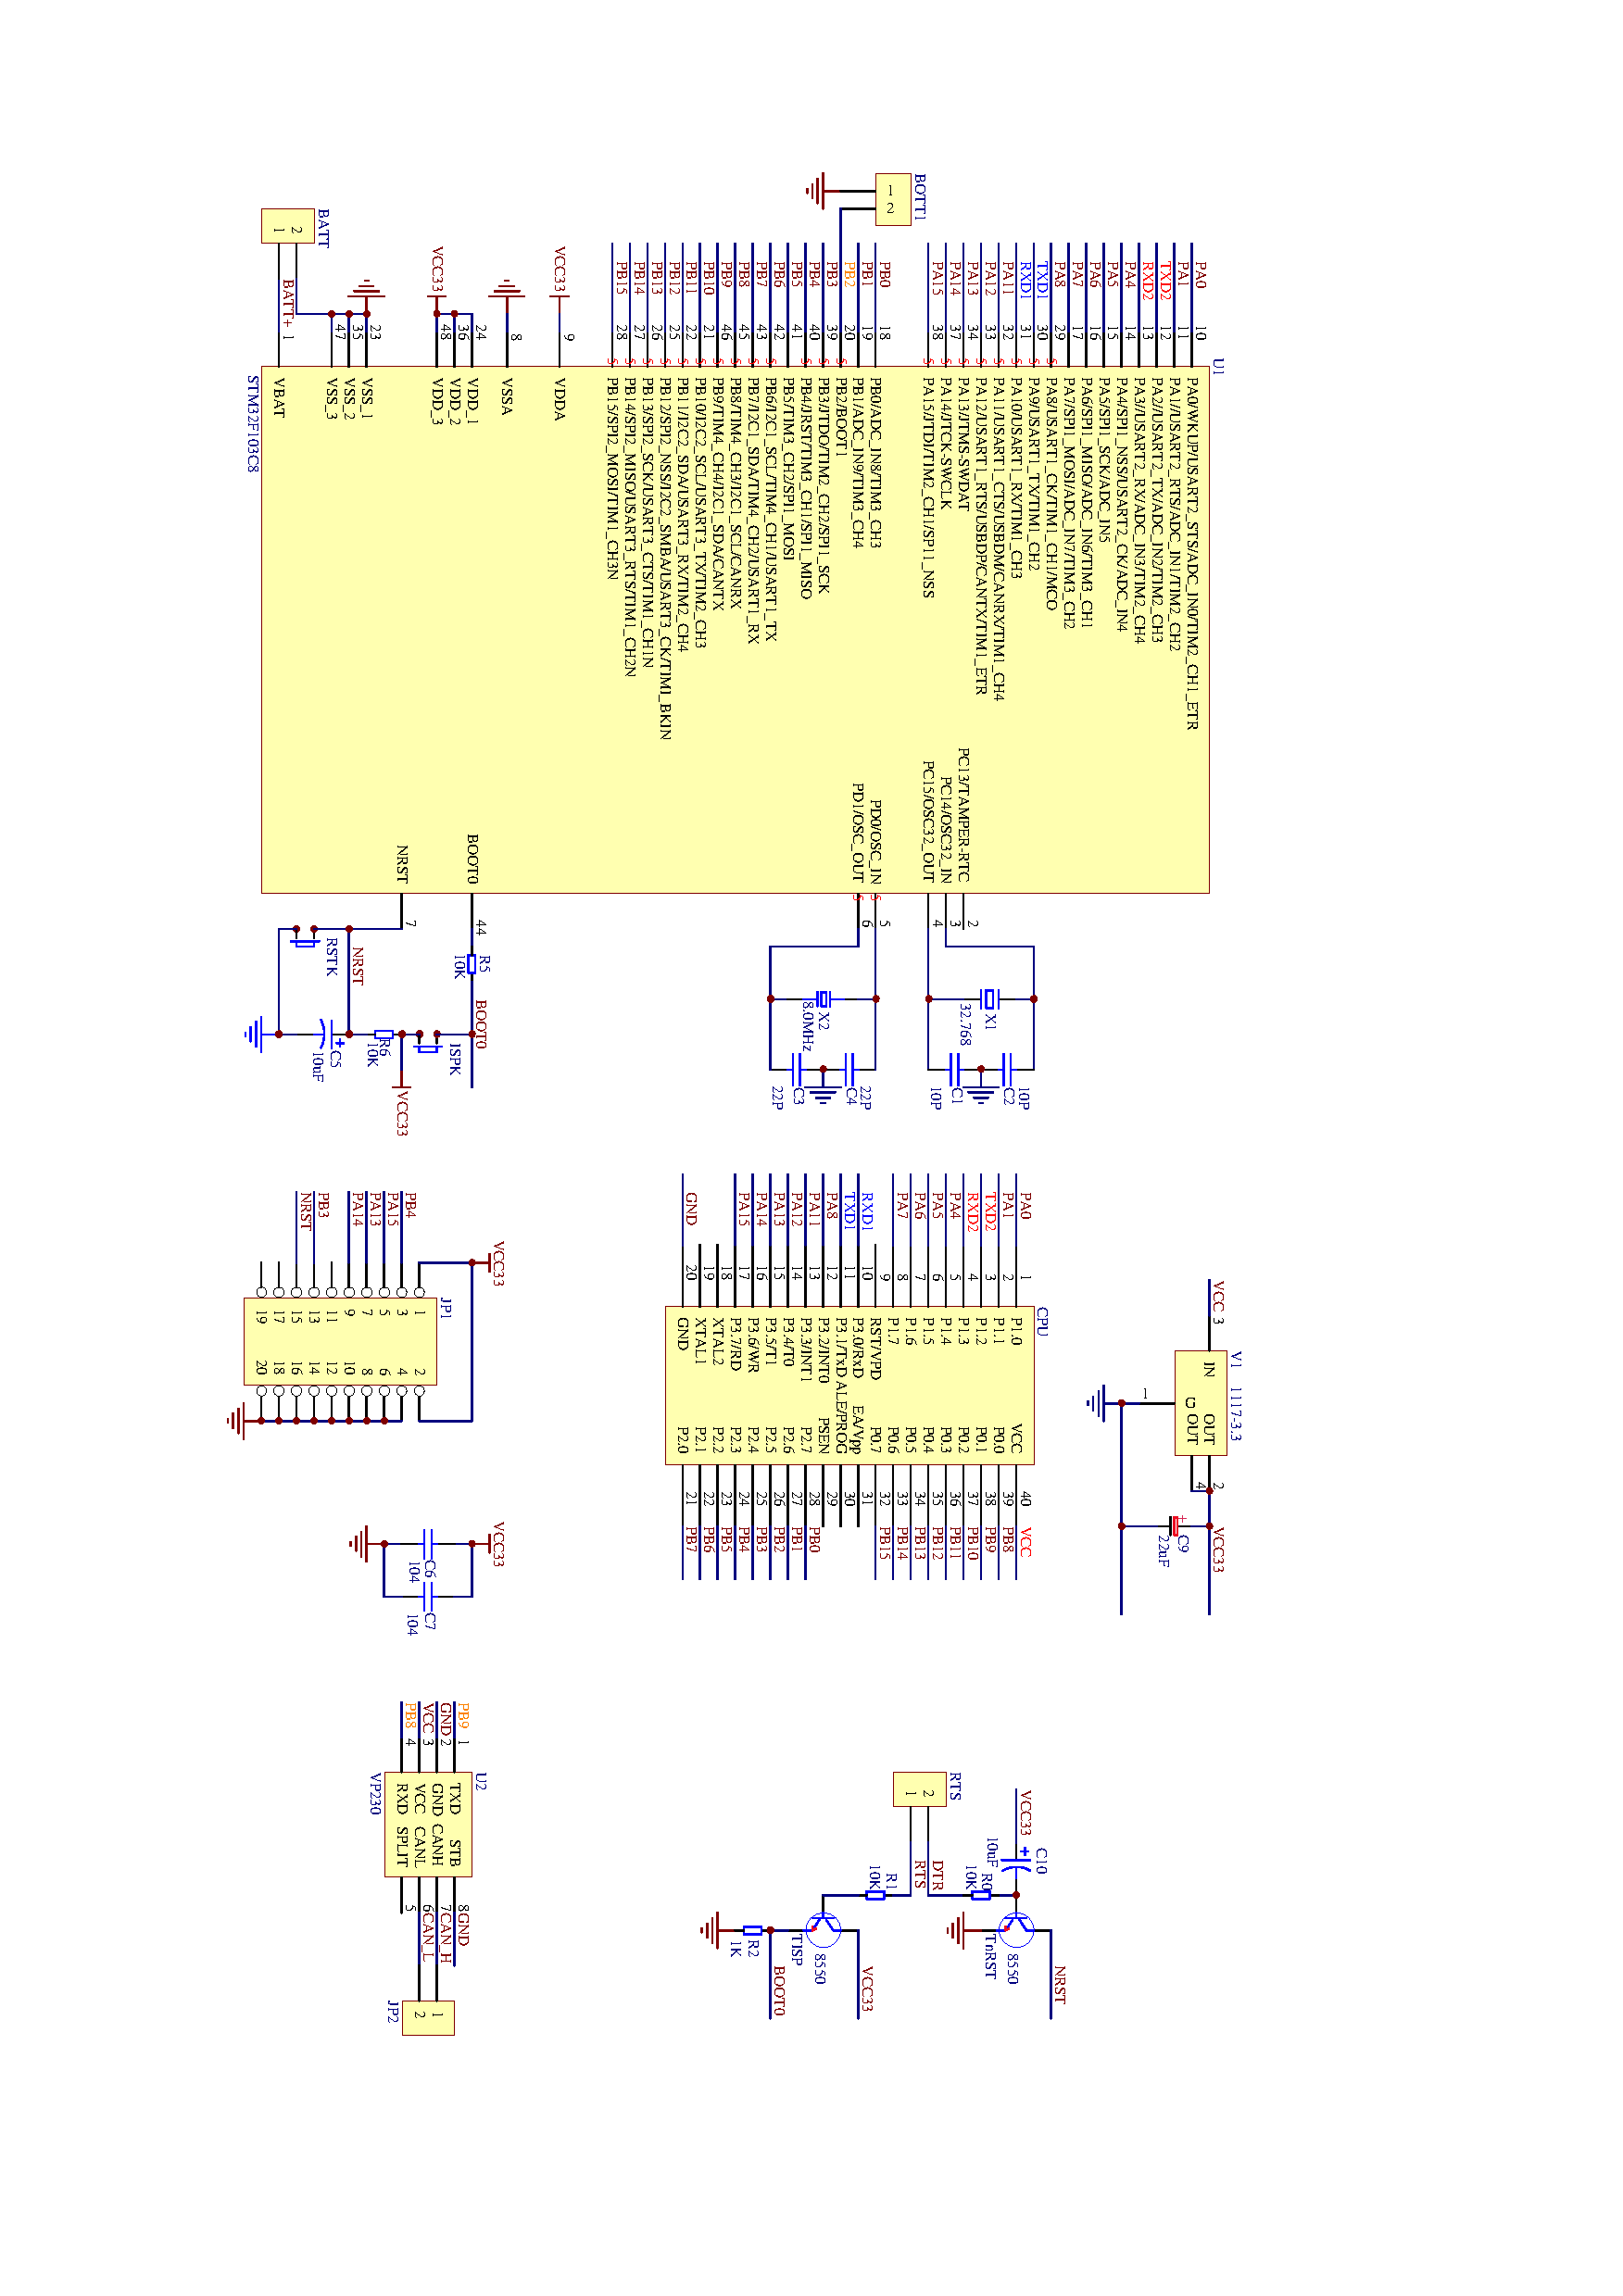
\includegraphics[width=0.7\textwidth]{figure/STM32.pdf}
\end{figure}
\newpage

\section{标志位代码}\label{标志位代码}
\begin{lstlisting}
uint8_t isflow=0;
uint8_t speed=0;
\end{lstlisting}

\section{按键进程代码}\label{按键进程代码}
\begin{lstlisting}
uint8_t last_state=0x00;
uint8_t KEY_Gets()
{
	uint8_t value = (uint8_t)(GPIO_ReadInputData(GPIOB)&0x00f0);
	uint8_t jump = (last_state^value)&value;
	last_state = value;
	return jump;
}
void LED_change()
{
	uint8_t value=0x00;
	SystickInit();
	while(1)
	{
		value=KEY_Gets();
		if(value&0x80)
			isflow+=1;
		if(value&0x40)
			speed+=1;
		OSTimeDlyHMSM(0,0,0,10);
	}
}
\end{lstlisting}
\section{流水进程代码}\label{流水进程代码}
\begin{lstlisting}
void LED_Sets(uint8_t k)
{
	uint16_t setValue;
	setValue = GPIO_ReadOutputData(GPIOB)&0x00ff;
	setValue |= (uint16_t)(1<<(k%8)) << 8;
	GPIO_Write(GPIOB,setValue);
}
void LED_flow()
{
	uint8_t count = 0;
	SystickInit();
	while(1)
	{
		if(isflow%2==0)
			LED_Sets(count++);
		OSTimeDlyHMSM(0,0,speed%3+1,0);
	}
}
\end{lstlisting}

\section{主函数代码}\label{主函数代码}
\subsection*{系统时钟初始化}
\begin{lstlisting}
static void SystickInit()
{
	RCC_ClocksTypeDef  rcc_clocks;  
	RCC_GetClocksFreq(&rcc_clocks);
	SysTick_Config(rcc_clocks.HCLK_Frequency / OS_TICKS_PER_SEC);
}
\end{lstlisting}

\subsection*{管脚的初始化}
\begin{lstlisting}
#define RCC_LED 	RCC_APB2Periph_GPIOB
#define PIN_KEY (GPIO_Pin_0|GPIO_Pin_1|GPIO_Pin_2|GPIO_Pin_3|\
	GPIO_Pin_4|GPIO_Pin_5|GPIO_Pin_6|GPIO_Pin_7)
#define PIN_LED (GPIO_Pin_8|GPIO_Pin_9|GPIO_Pin_10|GPIO_Pin_11|\
	GPIO_Pin_12|GPIO_Pin_13|GPIO_Pin_14|GPIO_Pin_15)
void LED_Init(void)
{
	GPIO_InitTypeDef GPIO_InitStructure;
	GPIO_InitStructure.GPIO_Pin = PIN_LED;
	GPIO_InitStructure.GPIO_Speed = GPIO_Speed_50MHz;
	GPIO_InitStructure.GPIO_Mode = GPIO_Mode_Out_PP;
	RCC_APB2PeriphClockCmd(RCC_LED, ENABLE);
	GPIO_Init(GPIOB, &GPIO_InitStructure);
}
void KEY_Init(void)
{
	GPIO_PinRemapConfig(GPIO_Remap_SWJ_Disable, ENABLE);
	GPIO_InitTypeDef GPIO_InitStructure;
	GPIO_InitStructure.GPIO_Pin=PIN_KEY;
	GPIO_InitStructure.GPIO_Speed=GPIO_Speed_50MHz;
	GPIO_InitStructure.GPIO_Mode=GPIO_Mode_IPU;
	RCC_APB2PeriphClockCmd(RCC_APB2Periph_AFIO,ENABLE);
	GPIO_Init(GPIOB,&GPIO_InitStructure);
}
void BSP_Init()
{
	LED_Init();
	KEY_Init();
}
\end{lstlisting}

\subsection*{操作系统系统的初始化、系统任务的创建和启动}
\begin{lstlisting}
static OS_STK task_LED_flow[STARTUP_TASK_STK_SIZE];
static OS_STK task_LED_change[STARTUP_TASK_STK_SIZE];
int main(void)
{
	BSP_Init();
	OSInit();
	OSTaskCreate(LED_flow,(void *)0,
		&task_LED_flow[STARTUP_TASK_STK_SIZE-1],
		STARTUP_TASK_PRIO);
	OSTaskCreate(LED_change,(void *)0,
		&task_LED_change[STARTUP_TASK_STK_SIZE-1],
		STARTUP_TASK_PRIO-1);
	OSStart();
}
\end{lstlisting}

\end{document}